
%(BEGIN_QUESTION)
% Copyright 2006, Tony R. Kuphaldt, released under the Creative Commons Attribution License (v 1.0)
% This means you may do almost anything with this work of mine, so long as you give me proper credit

Steam heaters are almost always of the {\it contra-flow} design, where the two fluids pass by each other in opposing directions:

$$\includegraphics[width=15.5cm]{i00335x01.eps}$$

This is very intentional.  If we were to have the fluids moving in the same direction, the exchanger would not be nearly as effective:

$$\includegraphics[width=15.5cm]{i00335x02.eps}$$

\vskip 10pt

Explain why this is, making reference to the equation ${dQ \over dt} = {kA {\Delta T} \over l}$ if possible.

\underbar{file i00335}
%(END_QUESTION)





%(BEGIN_ANSWER)

In the heat exchanger where the two fluids move in the same direction, the heated fluid can never exit the exchanger at a warmer temperature than the heating fluid exits.  With the contra-flow design, it can!

%(END_ANSWER)





%(BEGIN_NOTES)

The lesson to be learned here is that heat flow through conduction (through the exchanger tube walls) only occurs when there is a temperature differential, according to this equation:

$${dQ \over dt} = {kA {\Delta T} \over l}$$

If the heated fluid were somehow to exit the exchanger warmer than the heating fluid exits, heat flow near the tail end of the exchanger would be going the wrong way!

%INDEX% Physics, heat and temperature: heat exchangers

%(END_NOTES)


